% Supplementary material for main.tex: items moved out of the 6-page paper. Every number comes from the
% generated tables / figures (scripts/posthoc/s08_paper_assets.py and the s0x scripts). Compile main.tex first
% (equation numbers are read from main.aux via xr).
% Loaded BEFORE \documentclass. XeTeX (e.g. Tectonic): IEEEtran probes the Type-1 Times family 'ptm' while
% loading; map those probes silently. preamble.tex then sets TeX Gyre Termes / Cursor with fontspec.
\RequirePackage{iftex}
\ifXeTeX
  \DeclareFontFamily{TU}{ptm}{}
  \DeclareFontShape{TU}{ptm}{m}{n}{<->ssub * lmr/m/n}{}
  \DeclareFontShape{TU}{ptm}{m}{it}{<->ssub * lmr/m/it}{}
  \DeclareFontShape{TU}{ptm}{bx}{n}{<->ssub * lmr/bx/n}{}
  \DeclareFontShape{TU}{ptm}{bx}{it}{<->ssub * lmr/bx/it}{}
  \DeclareFontShape{TU}{ptm}{b}{n}{<->ssub * lmr/bx/n}{}
  \DeclareFontShape{TU}{ptm}{b}{it}{<->ssub * lmr/bx/it}{}
\fi

\documentclass[conference]{IEEEtran}
% Shared preamble for main.tex and supplement.tex (loaded after \documentclass).
\IEEEoverridecommandlockouts
\usepackage{cite}
\usepackage{amsmath,amssymb}
\usepackage{graphicx}
\usepackage{booktabs}
\usepackage{array}
\usepackage{url}
\ifXeTeX
  \usepackage{newtxmath}
  \usepackage{fontspec}
  \setmainfont{texgyretermes}[Extension=.otf, UprightFont=*-regular, BoldFont=*-bold,
    ItalicFont=*-italic, BoldItalicFont=*-bolditalic]
  \setmonofont{texgyrecursor}[Extension=.otf, UprightFont=*-regular, BoldFont=*-bold,
    ItalicFont=*-italic, BoldItalicFont=*-bolditalic]
\else
  % pdfLaTeX (e.g. Overleaf): IEEEtran's standard Times setup
  \usepackage[T1]{fontenc}
  \usepackage{newtxtext,newtxmath}
\fi
\usepackage{textcomp}
% generated by scripts/build_macros.py from result JSON - do not edit by hand
\newcommand{\NTradingDays}{3,161}
\newcommand{\DataStart}{2014-01-01}
\newcommand{\DataEnd}{2026-10-09}
\newcommand{\NEquityRowsM}{5.84}
\newcommand{\NEquityRows}{5,836,673}
\newcommand{\NSymbols}{3,748}
\newcommand{\NFOUnderlyings}{354}
\newcommand{\FOPerDayMin}{134}
\newcommand{\FOPerDayMax}{227}
\newcommand{\NStaleFiles}{92}
\newcommand{\NDelivOverlapDates}{12}
\newcommand{\NDelivOverlapMismatch}{0}
\newcommand{\NFOOverlapDays}{5}
\newcommand{\NAdjust}{1,442}
\newcommand{\NAdjustNSE}{841}
\newcommand{\NAdjustGap}{468}
\newcommand{\NAdjustDemerger}{133}
\newcommand{\NGOneChecks}{57}
\newcommand{\GOneMaxDiff}{0}
\newcommand{\NFeatures}{80}
\newcommand{\NBroadTrain}{2,102}
\newcommand{\NBroadVal}{978}
\newcommand{\NBroadTest}{1,796}
\newcommand{\NBroadTotal}{4,876}
\newcommand{\SuccBroad}{0.262}
\newcommand{\NAllTrain}{5,075}
\newcommand{\NAllVal}{1,979}
\newcommand{\NAllTest}{4,273}
\newcommand{\NAllTotal}{11,327}
\newcommand{\SuccAll}{0.249}
\newcommand{\NStrictTrain}{38}
\newcommand{\NStrictVal}{15}
\newcommand{\NStrictTest}{29}
\newcommand{\NStrictTotal}{82}
\newcommand{\SuccStrict}{0.241}
\newcommand{\TvHOneExp}{27.3}
\newcommand{\TvHOneRest}{26.2}
\newcommand{\TvHOneDiff}{+1.0}
\newcommand{\TvHOneP}{0.513}
\newcommand{\TvHOneQ}{0.94}
\newcommand{\TvHTwoExp}{26.7}
\newcommand{\TvHTwoRest}{26.8}
\newcommand{\TvHTwoP}{0.936}
\newcommand{\TvHThreeExp}{1.03}
\newcommand{\TvHThreeRest}{1.07}
\newcommand{\TvHThreeP}{0.801}
\newcommand{\ValAUCxgb}{0.492}
\newcommand{\ValAUCrf}{0.487}
\newcommand{\ValAUClogit}{0.528}
\newcommand{\ValAUCcomp}{0.506}
\newcommand{\XgbTrees}{14}
\newcommand{\XgbDepth}{2}
\newcommand{\HOneExp}{24.8}
\newcommand{\HOneRest}{24.9}
\newcommand{\HOneDiff}{\ensuremath{-}0.04}
\newcommand{\HOneP}{0.987}
\newcommand{\HOneQ}{0.987}
\newcommand{\HTwoExp}{23.5}
\newcommand{\HTwoRest}{26.3}
\newcommand{\HTwoDiff}{\ensuremath{-}2.8}
\newcommand{\HTwoP}{0.171}
\newcommand{\HTwoQ}{0.286}
\newcommand{\HThreeExp}{1.01}
\newcommand{\HThreeRest}{0.88}
\newcommand{\HThreeP}{0.384}
\newcommand{\HThreeQ}{0.480}
\newcommand{\AUCxgb}{0.460}
\newcommand{\AUCrf}{0.466}
\newcommand{\AUClogit}{0.468}
\newcommand{\AUCcomp}{0.526}
\newcommand{\HFourDiff}{\ensuremath{-}0.066}
\newcommand{\HFourSE}{0.023}
\newcommand{\HFourP}{0.005}
\newcommand{\HFourQ}{0.024}
\newcommand{\TopMLPrec}{22.4}
\newcommand{\TopCompPrec}{31.0}
\newcommand{\TopMLN}{165}
\newcommand{\TopP}{0.108}
\newcommand{\TopSpread}{\ensuremath{-}0.26}
\newcommand{\TopSpreadLo}{\ensuremath{-}1.29}
\newcommand{\TopSpreadHi}{+0.64}
\newcommand{\BrierRaw}{0.250}
\newcommand{\BrierCal}{0.195}
\newcommand{\WFAUC}{0.502}
\newcommand{\WFMonths}{46}
\newcommand{\NPHTwoDiff}{\ensuremath{-}5.6}
\newcommand{\NPHTwoP}{0.026}
\newcommand{\NPHTwoQ}{0.128}
\newcommand{\NPHFourDiff}{\ensuremath{-}0.039}
\newcommand{\NPHFourP}{0.141}
\newcommand{\BHm}{5}
\newcommand{\BaseRateTest}{0.248}
\newcommand{\TTwoDiff}{+0.8}
\newcommand{\TTwoP}{0.586}
\newcommand{\PowRuleN}{144}
\newcommand{\PowRuleDiff}{\ensuremath{-}0.2}
\newcommand{\PowRuleP}{0.978}
\newcommand{\LadBaseN}{159,972}
\newcommand{\LadBase}{26.7}
\newcommand{\LadAll}{24.9}
\newcommand{\LadAllDiff}{\ensuremath{-}1.9}
\newcommand{\LadAllP}{0.005}
\newcommand{\LadBroad}{24.8}
\newcommand{\LadComp}{41.4}
\newcommand{\LadCompN}{29}
\newcommand{\CagrAll}{\ensuremath{-}26.8}
\newcommand{\TradesAll}{2,736}
\newcommand{\MaxDDAll}{\ensuremath{-}68.6}
\newcommand{\CagrBroad}{\ensuremath{-}12.6}
\newcommand{\TradesBroad}{1,599}
\newcommand{\MaxDDBroad}{\ensuremath{-}39.2}
\newcommand{\CagrComp}{+6.0}
\newcommand{\TradesComp}{29}
\newcommand{\MaxDDComp}{\ensuremath{-}1.0}
\newcommand{\CagrML}{+4.3}
\newcommand{\TradesML}{157}
\newcommand{\MaxDDML}{\ensuremath{-}2.3}
\newcommand{\CagrNifty}{+9.7}
\newcommand{\SPAp}{0.77}
\newcommand{\RCp}{0.89}
\newcommand{\DSRtrials}{89}
\newcommand{\TrialsBefore}{67}
\newcommand{\TrialsTestRun}{22}
\newcommand{\TrialsThroughPSix}{89}
\newcommand{\PreregCommit}{15103f1}
\newcommand{\PreregTime}{08:54}
\newcommand{\LockHead}{ea49def}
\newcommand{\LockStart}{09:23}
\newcommand{\LockCommit}{359bcc7}
\newcommand{\LockCommitTime}{09:30}
\newcommand{\TostHOneLo}{\ensuremath{-}3.7}
\newcommand{\TostHOneHi}{+3.6}
\newcommand{\TostHOneP}{0.19}
\newcommand{\TostHTwoLo}{\ensuremath{-}6.2}
\newcommand{\TostHTwoHi}{+0.6}
\newcommand{\TostHTwoP}{0.65}
\newcommand{\TostNPHOneLo}{\ensuremath{-}1.9}
\newcommand{\TostNPHOneHi}{+7.2}
\newcommand{\TostNPHOneP}{0.59}
\newcommand{\TostNPHTwoLo}{\ensuremath{-}9.8}
\newcommand{\TostNPHTwoHi}{\ensuremath{-}1.5}
\newcommand{\TostNPHTwoP}{0.93}
\newcommand{\MDEHOne}{6.26}
\newcommand{\MDEHTwo}{5.71}
\newcommand{\ExpN}{47}
\newcommand{\ExpRemoved}{331}
\newcommand{\ExpDiff}{\ensuremath{-}1.4}
\newcommand{\ExpP}{0.572}
\newcommand{\ExpPMin}{0.516}
\newcommand{\PSIpcr}{0.55}
\newcommand{\PSIclient}{0.31}
\newcommand{\PSInModerate}{7}
\newcommand{\PSInLarge}{2}
\newcommand{\BrierConstVal}{0.188}
\newcommand{\BrierConstTest}{0.187}
\newcommand{\IncompleteBroad}{4}
\newcommand{\GapEvents}{165}
\newcommand{\GapTrades}{157}
\newcommand{\GapSlotsFull}{8}
\newcommand{\RoundTrip}{0.58}
\newcommand{\RTLarge}{0.45}
\newcommand{\RTSmall}{0.75}
\newcommand{\AvgWin}{+4.74}
\newcommand{\AvgLoss}{\ensuremath{-}1.85}
\newcommand{\WinLossSpread}{6.59}
\newcommand{\BreakEven}{8.8}
\newcommand{\BEHOneDiff}{\ensuremath{-}0.0}
\newcommand{\BEHOneLo}{\ensuremath{-}4.4}
\newcommand{\BEHOneHi}{+4.3}
\newcommand{\BEHOneBLo}{\ensuremath{-}5.3}
\newcommand{\BEHOneBHi}{+4.7}
\newcommand{\BEHOneN}{1265}
\newcommand{\BEHTwoDiff}{\ensuremath{-}2.8}
\newcommand{\BEHTwoLo}{\ensuremath{-}6.8}
\newcommand{\BEHTwoHi}{+1.2}
\newcommand{\BEHTwoBLo}{\ensuremath{-}8.3}
\newcommand{\BEHTwoBHi}{+2.1}
\newcommand{\BEHTwoN}{924}
\newcommand{\BENPHOneDiff}{+2.6}
\newcommand{\BENPHOneLo}{\ensuremath{-}2.8}
\newcommand{\BENPHOneHi}{+8.1}
\newcommand{\BENPHOneBLo}{\ensuremath{-}2.8}
\newcommand{\BENPHOneBHi}{+7.9}
\newcommand{\BENPHOneN}{899}
\newcommand{\BENPHTwoDiff}{\ensuremath{-}5.6}
\newcommand{\BENPHTwoLo}{\ensuremath{-}10.6}
\newcommand{\BENPHTwoHi}{\ensuremath{-}0.7}
\newcommand{\BENPHTwoBLo}{\ensuremath{-}12.3}
\newcommand{\BENPHTwoBHi}{+0.7}
\newcommand{\BENPHTwoN}{617}
\newcommand{\BEMLDiff}{\ensuremath{-}2.7}
\newcommand{\BEMLLo}{\ensuremath{-}9.4}
\newcommand{\BEMLHi}{+4.1}
\newcommand{\BEMLBLo}{\ensuremath{-}13.8}
\newcommand{\BEMLBHi}{+7.3}
\newcommand{\BEMLN}{165}
\newcommand{\BECompTopDiff}{+7.0}
\newcommand{\BECompTopLo}{+0.6}
\newcommand{\BECompTopHi}{+13.4}
\newcommand{\BECompTopBLo}{+0.8}
\newcommand{\BECompTopBHi}{+15.0}
\newcommand{\BECompTopN}{226}
\newcommand{\BECompRuleDiff}{+16.8}
\newcommand{\BECompRuleLo}{\ensuremath{-}1.2}
\newcommand{\BECompRuleHi}{+34.9}
\newcommand{\BECompRuleBLo}{\ensuremath{-}10.0}
\newcommand{\BECompRuleBHi}{+46.3}
\newcommand{\BECompRuleN}{29}
\newcommand{\BEnBelow}{3}
\newcommand{\SpecOneN}{54}
\newcommand{\SpecOnePred}{89}
\newcommand{\SpecOneSig}{15}
\newcommand{\SpecOneSigPct}{28}
\newcommand{\SpecOneOpp}{0}
\newcommand{\SpecOneBH}{3}
\newcommand{\SpecOneMedian}{+2.36}
\newcommand{\SpecOneMax}{5.05}
\newcommand{\SpecOneCIAbove}{4}
\newcommand{\SpecOneFrozen}{\ensuremath{-}0.04}
\newcommand{\SpecOneRank}{49}
\newcommand{\SpecTwoN}{18}
\newcommand{\SpecTwoPred}{94}
\newcommand{\SpecTwoSig}{3}
\newcommand{\SpecTwoSigPct}{17}
\newcommand{\SpecTwoOpp}{0}
\newcommand{\SpecTwoBH}{0}
\newcommand{\SpecTwoMedian}{\ensuremath{-}2.24}
\newcommand{\SpecTwoMax}{4.44}
\newcommand{\SpecTwoCIAbove}{0}
\newcommand{\SpecTwoFrozen}{\ensuremath{-}2.81}
\newcommand{\SpecTwoRank}{6}
\newcommand{\BFOneUni}{17.88}
\newcommand{\BFNPOneUni}{9.31}
\newcommand{\BFOneSkep}{2.27}
\newcommand{\BFNPOneSkep}{1.27}
\newcommand{\BFOneLogDef}{8.41}
\newcommand{\BFNPOneLogDef}{4.49}
\newcommand{\BFOneLogSkep}{2.32}
\newcommand{\BFNPOneLogSkep}{1.43}
\newcommand{\BFTwoUni}{7.65}
\newcommand{\BFNPTwoUni}{1.31}
\newcommand{\BFTwoSkep}{1.05}
\newcommand{\BFNPTwoSkep}{0.23}
\newcommand{\BFTwoLogDef}{3.63}
\newcommand{\BFNPTwoLogDef}{0.67}
\newcommand{\BFTwoLogSkep}{1.13}
\newcommand{\BFNPTwoLogSkep}{0.30}
\newcommand{\EOneBOne}{+0.008}
\newcommand{\EOneBOneLo}{\ensuremath{-}0.237}
\newcommand{\EOneBOneHi}{+0.254}
\newcommand{\EOneBOneP}{0.946}
\newcommand{\EOneBTwo}{\ensuremath{-}0.225}
\newcommand{\EOneBTwoLo}{\ensuremath{-}0.592}
\newcommand{\EOneBTwoHi}{+0.142}
\newcommand{\EOneBTwoP}{0.229}
\newcommand{\EOneBThree}{+0.246}
\newcommand{\EOneBThreeLo}{\ensuremath{-}0.130}
\newcommand{\EOneBThreeHi}{+0.622}
\newcommand{\EOneBThreeP}{0.200}
\newcommand{\ETwoBOne}{\ensuremath{-}0.129}
\newcommand{\ETwoBOneLo}{\ensuremath{-}0.361}
\newcommand{\ETwoBOneHi}{+0.102}
\newcommand{\ETwoBOneP}{0.273}
\newcommand{\ETwoBTwo}{+0.185}
\newcommand{\ETwoBTwoLo}{+0.006}
\newcommand{\ETwoBTwoHi}{+0.364}
\newcommand{\ETwoBTwoP}{0.043}
\newcommand{\ETwoBThree}{\ensuremath{-}0.186}
\newcommand{\ETwoBThreeLo}{\ensuremath{-}0.435}
\newcommand{\ETwoBThreeHi}{+0.063}
\newcommand{\ETwoBThreeP}{0.142}
\newcommand{\EMonthMatches}{exactly}
\newcommand{\FYears}{12}
\newcommand{\FYearsSig}{0}
\newcommand{\FFirstYear}{2015}
\newcommand{\FLastYear}{2026}
\newcommand{\GTieShareLoss}{0.12}
\newcommand{\GTieExplained}{0.1}
\newcommand{\GDayOneBO}{15.0}
\newcommand{\GDayOneNB}{10.3}
\newcommand{\GRangeBO}{1.07}
\newcommand{\GRangeNB}{0.95}
\newcommand{\GGapBO}{0.11}
\newcommand{\GGapNB}{0.05}
\newcommand{\GATRBO}{2.55}
\newcommand{\GATRNB}{2.68}
\newcommand{\GAgree}{100.0}
\newcommand{\placeboDraws}{1,000}
\newcommand{\placeboActual}{\ensuremath{-}0.04}
\newcommand{\placeboMean}{+1.65}
\newcommand{\placeboSD}{1.97}
\newcommand{\placeboP}{0.795}
\newcommand{\placeboPct}{20}
\newcommand{\PSevenActual}{+1.05}
\newcommand{\PSevenDraws}{20}
\newcommand{\PSevenGE}{0}

\raggedbottom

\usepackage{xr}
\externaldocument{main}
\renewcommand{\thetable}{S\arabic{table}}
\renewcommand{\thefigure}{S\arabic{figure}}

\begin{document}
\title{Supplementary Material:\\Do Delivery and Futures-Positioning Footprints Predict Breakout Success?}
\author{\IEEEauthorblockN{Fazil T, Faizur Rahman S, Suhail Ahmed S, Jeyavim Sherin R C}
\IEEEauthorblockA{Dept.\ of CSE (AI \& ML), Hindustan Institute of Technology and Science, Chennai, India}}
\maketitle

This supplement holds the tables and figures moved out of the main paper for length. Tables~\ref{tab:audit}--\ref{tab:robust} and Fig.~\ref{fig:forest} are post-hoc (designed after
the test set was opened on 10 October 2026, 09:23 IST); Table~\ref{tab:backtestsfull} and Fig.~\ref{fig:cagr} show
pre-registered test results.

% generated by scripts/posthoc/s08_paper_assets.py from result JSON - do not edit by hand
\begin{table}[t]
\centering
\caption{Supplementary audit of the locked test evaluation}
\label{tab:audit}
\footnotesize
\setlength{\tabcolsep}{4pt}
\begin{tabular}{@{}>{\raggedright\arraybackslash}p{3.0cm}l>{\raggedright\arraybackslash}p{3.4cm}@{}}
\toprule
\textbf{Check} & \textbf{Label} & \textbf{Result} \\
\midrule
MDE, H1 / H2 (80\%, $\alpha$=.05) & PRE-REG. & 6.26 / 5.71 pp \\
Cost break-even $d^*$ & POST-HOC & 0.58\% / 6.59 pp = 8.8 pp \\
TOST $\pm$2 pp, H1 (full) & POST-HOC & 90\% CI [\ensuremath{-}3.7, +3.6], $p$=0.19 \\
TOST $\pm$2 pp, H2 (full) & POST-HOC & 90\% CI [\ensuremath{-}6.2, +0.6], $p$=0.65 \\
H1 excl.\ 5 sessions pre-expiry & POST-HOC & \ensuremath{-}1.4 pp, $p$=0.57 (331 removed) \\
PSI $>$0.25 among top-10 SHAP & POST-HOC & client\_fut\_idx\_cot 0.31, log\_pcr\_oi 0.55 \\
Brier: constant / calibrated XGB & POST-HOC & 0.1879 / 0.1953 \\
Incomplete labels (last 10 days) & PRE-REG.\ rule & 4 BROAD events excluded \\
ML top decile: events vs trades & PRE-REG.\ rule & 165 vs 157 (slots full) \\
\bottomrule
\end{tabular}
\par\smallskip\parbox{0.98\linewidth}{\scriptsize\raggedright POST-HOC rows were designed after the test set was opened (10 Oct 2026, 09:23 IST). Brier constant uses the validation base rate (no test information).}
\end{table}

% generated by scripts/posthoc/s08_paper_assets.py from result JSON - do not edit by hand
\begin{table*}[t]
\centering
\caption{Post-hoc robustness on the test set}
\label{tab:robust}
\footnotesize
\setlength{\tabcolsep}{4pt}
\begin{tabular}{llll}
\toprule
\textbf{Hyp.} & \textbf{Spec./prior/term} & \textbf{Value} & \textbf{Reading (full test)} \\
\midrule
\multicolumn{4}{l}{\textit{Specification curve (barrier $\times$ horizon $\times$ threshold $\times$ event set)}} \\
H1 & 54 specs & 15 sig.\ (28\%), 0 opposite & median +2.36 pp; frozen \ensuremath{-}0.04 pp \\
H2 & 18 specs & 3 sig.\ (17\%), 0 opposite & median \ensuremath{-}2.24 pp; frozen \ensuremath{-}2.81 pp \\
\midrule
\multicolumn{4}{l}{\textit{Bayes factor BF$_{01}$ (BROAD, full test / without pilot)}} \\
H1 & Beta(1,1) & 17.88 / 9.31 & strong evidence for H0 (no difference) \\
H1 & skeptical Beta & 2.27 / 1.27 & anecdotal evidence for H0 (no difference) \\
H1 & logOR$\sim$N(0,1) & 8.41 / 4.49 & moderate evidence for H0 (no difference) \\
H1 & logOR$\sim$N(0,0.25$^2$) & 2.32 / 1.43 & anecdotal evidence for H0 (no difference) \\
H2 & Beta(1,1) & 7.65 / 1.31 & moderate evidence for H0 (no difference) \\
H2 & skeptical Beta & 1.05 / 0.23 & anecdotal evidence for H0 (no difference) \\
H2 & logOR$\sim$N(0,1) & 3.63 / 0.67 & moderate evidence for H0 (no difference) \\
H2 & logOR$\sim$N(0,0.25$^2$) & 1.13 / 0.30 & anecdotal evidence for H0 (no difference) \\
\midrule
\multicolumn{4}{l}{\textit{Logit model, Eq.~(\ref{eq:logit}), on the test set, BROAD, two-way (date $\times$ symbol) clustered SE}} \\
H1 & $\beta_1$ deliv\_exp & +0.008 [\ensuremath{-}0.237, +0.254] & $p$=0.946 \\
H1 & $\beta_2$ pos & \ensuremath{-}0.225 [\ensuremath{-}0.592, +0.142] & $p$=0.229 \\
H1 & $\beta_3$ deliv\_exp:pos & +0.246 [\ensuremath{-}0.130, +0.622] & $p$=0.200 \\
H2 & $\beta_1$ div & \ensuremath{-}0.129 [\ensuremath{-}0.361, +0.102] & $p$=0.273 \\
H2 & $\beta_2$ dz & +0.185 [+0.006, +0.364] & $p$=0.043 \\
H2 & $\beta_3$ div:dz & \ensuremath{-}0.186 [\ensuremath{-}0.435, +0.063] & $p$=0.142 \\
\bottomrule
\end{tabular}
\par\smallskip\parbox{0.95\linewidth}{\scriptsize\raggedright ALL POST-HOC. Specs overlap and are not corrected for multiplicity. BF$_{01}>1$ favours no difference; it shrinks towards 1 under skeptical priors that let the alternative predict small effects. Month-clustered SEs reproduce the locked P6 values exactly; STRICT logits are not estimable ($n=28$, separation).}
\end{table*}

% generated by scripts/posthoc/s08_paper_assets.py from result JSON - do not edit by hand
\begin{table*}[t]
\centering
\caption{Costed test-set backtests (2023-01 to 2026-10)}
\label{tab:backtests}
\footnotesize
\setlength{\tabcolsep}{4pt}
\begin{tabular}{lrrrrrrl}
\toprule
\textbf{Strategy} & \textbf{Trades} & \textbf{CAGR} & \textbf{Sharpe} & \textbf{MaxDD} & \textbf{Hit\%} & \textbf{PF} &  \\
\midrule
B1 all breakouts & 2,736 & \ensuremath{-}26.8 & \ensuremath{-}4.02 & \ensuremath{-}68.6 & 31.5 & 0.59 & ok \\
B2 STRICT & 29 & +5.7 & \ensuremath{-}0.47 & \ensuremath{-}0.5 & 34.5 & 0.72 & n$<$30 \\
B4 STRICT ML top decile & 1 & -- & -- & -- & 0.0 & 0.00 & n$<$30 \\
B2b BROAD & 1,599 & \ensuremath{-}12.6 & \ensuremath{-}3.25 & \ensuremath{-}39.2 & 32.1 & 0.60 & ok \\
B3b BROAD composite & 29 & +6.0 & \ensuremath{-}0.01 & \ensuremath{-}1.0 & 41.4 & 1.04 & n$<$30 \\
B4b BROAD ML top decile & 157 & +4.3 & \ensuremath{-}0.85 & \ensuremath{-}2.3 & 33.1 & 0.64 & ok \\
\midrule
Nifty 500 (benchmark) & -- & +9.7 & 0.32 & \ensuremath{-}18.8 & -- & -- &  \\
\bottomrule
\end{tabular}
\par\smallskip\parbox{0.95\linewidth}{\scriptsize\raggedright PRE-REGISTERED (P6, run once). Full Indian costs and slippage; max.\ 20 positions. Hansen SPA $p$=0.77, White RC $p$=0.89; deflated Sharpe $\approx 0$ for all (N = 89 results-log rows at the time of the run, of which 67 were logged before the test run started).}
\end{table*}



\begin{figure}[t]
\centering
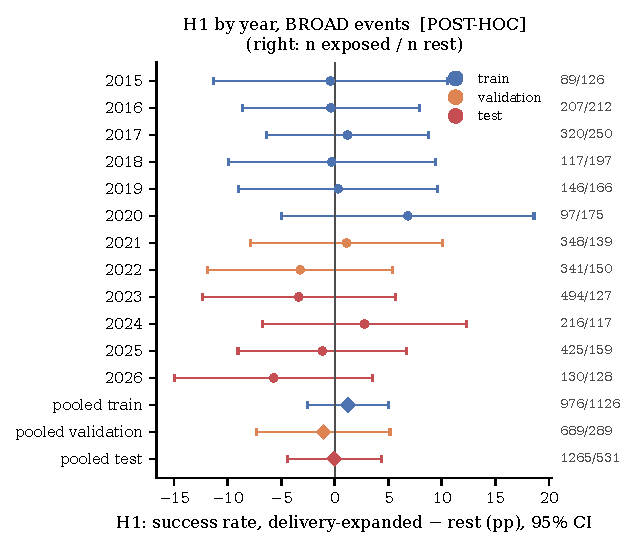
\includegraphics[width=\columnwidth]{figs/fig_h1_forest.pdf}
\caption{Post-hoc H1 effect by calendar year with 95\% CIs, coloured by split.}
\label{fig:forest}
\end{figure}


\begin{figure}[t]
\centering
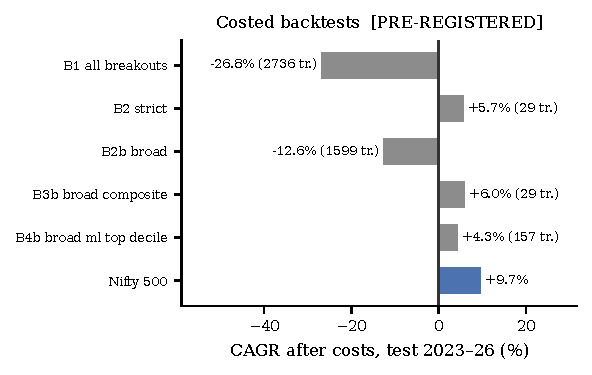
\includegraphics[width=\columnwidth]{figs/fig_cagr.pdf}
\caption{Test-period CAGR after Indian costs (pre-registered backtests).}
\label{fig:cagr}
\end{figure}

\end{document}
